\begin{frame}
	\frametitle{Custos de Curto Prazo}

	O objectivo de uma empresa \'e maximizar o seu lucro, dadas as condi\c c\~oes de mercado de factores e as de mercado do produto onde a sua actividade se desenvolve. \pause

	\vspace{1cm}

	Em geral, \[\text{Lucro}=\text{Receitas Totais}-\text{Custos Totais}\]
	
\end{frame}

\begin{frame}
	\frametitle{Custos a curto-prazo}
	O custo total \'e obtido adicionando:
	\begin{itemize}
		\item Custo fixo (\(CF\)), que n\~ao depende da quantidade produzida, e que \'e o custo dos factores de produ\c c\~ao fixos (\(K\))
		\item Custo vari\'avel (\(CV\)), que depende da quantidade de factor vari\'avel contratado (\(L\)), o que, por sua vez, determina a quantidade produzida.
	\end{itemize}
	\[CT = C(Q) = CV + CF\]

\end{frame}

\begin{frame}
	\frametitle{Fun\c c\~ao de Produ\c c\~ao e Custos}
	No mercado dos factores, admitamos: Custo de $K$ instalado $=60$; custo de cada unidade de trabalho = $250$

	\begin{center}
		\begin{tabular}{ccccc}
			$L$ & $Q$ & $CF$ & $CV$ & $CT$ \\ \hline \hline
			0 & 0 & 60 & 0 & 60 \\
			1 & 20 & 60 & 250 & 310 \\
			2 & 50 & 60 & 500 & 560 \\
			3 & 85 & 60 & 750 & 810 \\
			4 & 114 & 60 & 1,000 & 1,060 \\
			5 & 140 & 60 & 1,250 & 1,310 \\
			6 & 159 & 60 & 1,500 & 1,560 \\
			7 & 169 & 60 & 1,750 & 1,810 \\
			8 & 164 & 60 & 2,000 & 2,060
		\end{tabular}
	\end{center}
\end{frame}

\begin{frame}
	\frametitle{$CT,CV,CF$}
	\begin{center}
		\begin{tikzpicture}[
			scale = 1,
			every node/.style = {scale =1},
			declare function = {
				cv(\x) = \x - (1/5)*\x^2 + (1/30)*\x^3;
				cf(\x) = 1;
				ct(\x) = cv(\x) + cf(\x);
			}
		]

		\draw[->,thick] (-0.1,0) -- (5.1,0) node[below]{$Q$};
		\draw[->,thick] (0,-0.1) -- (0,5.1) node[left]{$CT,CV,CF$};

		\onslide<3->{
			\draw[red,domain=0:5,variable=\x] plot (\x,{cv(\x)});
			\draw[red](5,{cv(5)})node[right]{CV};
		}
		\onslide<2->{
			\draw[blue,domain=0:5,variable=\x] plot (\x,{cf(\x)});
			\draw[blue](5,{cf(5)})node[right]{CF};
		}
		\onslide<4->{
			\draw[domain=0:5,variable=\x] plot (\x,{ct(\x)});
			\draw(5,{ct(5)})node[right]{CT};	
		}

		\end{tikzpicture}
	\end{center}
\end{frame}

\begin{frame}
	\frametitle{Custo Marginal}
	Custo marginal - Varia\c c\~ao do custo total quando se produz uma unidade adicional do produto (graficamente, identifica-se como o declive da recta tangente \`a curva de custos num ponto) \[Cmg=\frac{\Delta CT}{\Delta Q}=\frac{d CT}{d Q}\]
\end{frame}

\begin{frame}
	\frametitle{Custo Marginal}
	\begin{center}
		{
		\renewcommand{\arraystretch}{1.1}
		\begin{tabular}{ccccccc}
			$L$ & $Q$ & $CT$ & $CMg$ & $MPL$ & $APL$ & Etapa \\\hline \hline
			0 & 0 & 60 & & & & \\
			1 & 20 & 310 & 12.5 & 20 & 20 & I \\
			2 & 50 & 560 & 8.33 & 30 & 25 & I \\
			3 & 85 & 810 & 7.14 & 35 & 28.33 & I \\
			4 & 114 & 1060 & 8.62 & 29 & 28.5 & I \\
			5 & 140 & 1310 & 9.62 & 26 & 28 & II \\
			6 & 159 & 1560 & 13.16 & 19 & 26.5 & II \\
			7 & 169 & 1810 & 25 & 10 & 24.14 & II \\
			8 & 164 &  &  & -5  &  & III
		\end{tabular}
		}
	\end{center}
\end{frame}

\begin{frame}
	\frametitle{Custo Marginal}
	\begin{center}
		{
		\renewcommand{\arraystretch}{1.1}
		\begin{tabular}{ccccccc}
			$L$ & $Q$ & $CT$ & $CMg$ & $MPL$ & $APL$ & Etapa \\\hline \hline
			0 & 0 & 60  & & & & \\
			1 & 20 & 310 & 12.5 & 20 & 20 & I \\
			2 & 50 & 560 & 8.33 & 30 & 25 & I \\
			3 & 85 & 810 & 7.14 & 35 & 28.33 & I \\
			4 & 114 & 1060 & 8.62 & 29 & 28.5 & I \\
			5 & 140 & 1310 & 9.62 & 26 & \cellcolor{green!40!white}28 & II \\
			6 & 159 & 1560 & 13.16 & 19 & \cellcolor{green!40!white}26.5 & II \\
			7 & 169 & 1810 & 25 & 10 & \cellcolor{green!40!white}24.14 & II \\
			8 & 164 &  &  &  &  & III
		\end{tabular}
		}
	\end{center}
\end{frame}

\begin{frame}
	\frametitle{CMg: Observa\c c\~oes}
	\begin{itemize}
		\item O $CMg$ \'e fun\c c\~ao do n\'ivel do produto... \pause
		\item O $CMg$ \'e independente do custo fixo, pelo que pode calcular-se a partir de $CT$ ou a partir de $CV$ \pause
		\item O $CMg$ \'e crescente sempre que MPL \'e decrescente (Lei dos Rendimentos Marginais Decrescentes)\pause
		\item O $CMg$ \'e crescente na segunda etapa do processo produtivo, logo: \pause
		\begin{itemize}
			\item Na zona econ\'omica de explora\c c\~ao, onde se devem localizar as escolhas \'optimas de produ\c c\~ao, o $CMg$ \'e crscente! \'E por isso que a curva de oferta \'e positivamente inclinada
		\end{itemize}
	\end{itemize}
\end{frame}

\begin{frame}
	\frametitle{$CT,CV,CF$}
	\begin{center}
		\begin{tikzpicture}[
			scale = 1,
			every node/.style = {scale =1},
			declare function = {
				cv(\x) = \x - (1/4)*\x^2 + (1/25)*\x^3;
				cf(\x) = 1;
				ct(\x) = cv(\x) + cf(\x);
				cmg(\x) = 1 - (2/4)*\x + (3/25)*\x^2;
			}
		]

		\draw[->,thick] (-0.1,0) -- (5.1,0) node[below]{$Q$};
		\draw[->,thick] (0,-0.1) -- (0,5.1) node[left]{$CT,CV,CF$};

		\draw[red,thick,domain=0:5,variable=\x] plot (\x,{cv(\x)});
		\draw[blue,thick,domain=0:5,variable=\x] plot (\x,{cmg(\x)});
		
		\draw[red](5,{cv(5)})node[right]{CV};
		\draw[blue](5,{cmg(5)})node[right]{CMg};

		\draw[dashed] ({25/12},0) -- ({25/12},{cv(25/12)});
		
		\end{tikzpicture}
	\end{center}
\end{frame}

\begin{frame}
	\frametitle{Custos M\'edios}
	\pause
	\begin{itemize}
		\item \textbf{Custo fixo m\'edio:} Custo fixo por unidade produzida: $CFM=\frac{CF}{Q}$. O $CFM$ \'e sempre decrescente. \pause
		\item \textbf{Custo vari\'avel m\'edio:} Custo vari\'avel por unidade produzida: $CVM=\frac{CV}{Q}$. A forma t\'ipica do $CVM$ \'e a de um $U$, tal como a do $CMg$ \pause
		\item \textbf{Custo total m\'edio:} Custo total por unidade produzida: $CTM=\frac{CT}{Q}$ o $CTM$ (ou $CM$) \'e igual ao somat\'orio das suas componentes $CFM+CVM$. 

		A forma t\'ipica do $CM$ \'e a de um $U$, tal como a do $CMg$ e do $CVM$.
	\end{itemize}
\end{frame}

\begin{frame}
	\frametitle{$CVM$, $CTM$ e $CMg$}
	\begin{center}
		{
		\renewcommand{\arraystretch}{1.1}
		\begin{tabular}{ccccccc}
			$L$ & $Q$ & $CT$ & $CMg$ & $CVM$ & $CTM$ & Etapa \\\hline \hline
			0 & 0 & 60  & & & & \\
			1 & 20 & 310 & \cellcolor{yellow!80!red} 12.5 & 12.50 & 15.50 & I \\
			2 & 50 & 560 & \cellcolor{yellow!80!red}8.33 & 10 & 11.20 & I \\
			3 & 85 & 810 & \cellcolor{yellow!80!red}7.14 & 8.82 & 9.53 & I \\
			4 & 114 & 1060 & \cellcolor{yellow!80!red}8.62 & \cellcolor{green!80!white}8.77 & 9.30 & I \\
			5 & 140 & 1310 & 9.62 & 8.93 & 9.36 & II \\
			6 & 159 & 1560 & 13.16 & 9.43 & 9.81 & II \\
			7 & 169 & 1810 & 25 & 10.36 & 10.71 & II \\
			8 & 164 &  &  &  &  & III
		\end{tabular}
		}
	\end{center}
\end{frame}

\begin{frame}
	\frametitle{$CVM$, $CTM$ e $CMg$}
	A partir do quadro verifica-se que:
	\begin{itemize}
		\item $CTM$ est\'a sempre acima de $CVM$ (a diferen\c ca \'e $CFM$)
		\item $CTM$ e $CVM$ s\~ao decrescentes, enquanto o $CMg$ lhes for inferior: $CMg$ intersecta $CTM$ e $CVM$ nos seus m\'inimos
	\end{itemize}
\end{frame}

\begin{frame}
	\frametitle{$CT,CV,CF$}
	\begin{center}
		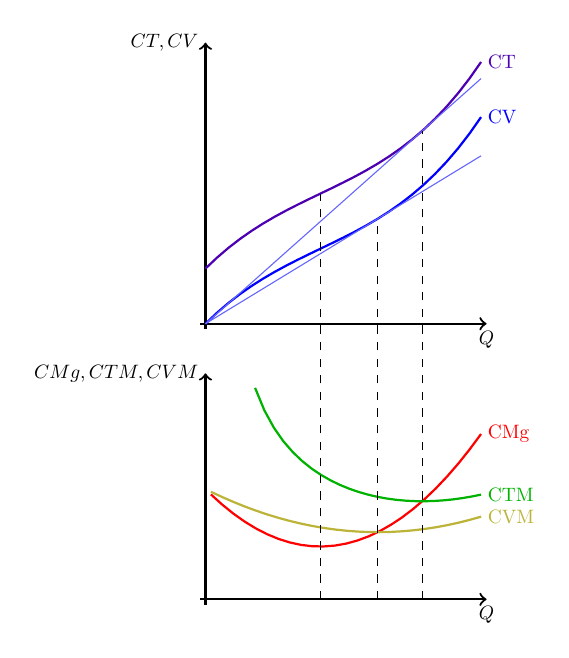
\begin{tikzpicture}[
			scale = 0.7,
			every node/.style = {scale =0.7},
			declare function = {
				cv(\x) = \x - (1/4)*\x^2 + (1/25)*\x^3;
				cf(\x) = 1;
				ct(\x) = cv(\x) + cf(\x);
				cmg(\x) = 1 - (2/4)*\x + (3/25)*\x^2;
				ctm(\x) = ct(\x)/\x;
				cvm(\x) = cv(\x)/\x;
			}
		]

		\draw[->,thick] (-0.1,0) -- (5.1,0) node[below]{$Q$};
		\draw[->,thick] (0,-0.1) -- (0,5.1) node[left]{$CT,CV$};

		\onslide<2->{
			\draw[blue,thick,domain=0:5,variable=\x] plot (\x,{cv(\x)});
			\draw[blue!60!white,domain=0:5,variable=\x] plot (\x,{\x*cvm(25/8)});	
			\draw[blue](5,{cv(5)})node[right]{CV};
		}

		\onslide<3->{
			\draw[blue!70!red,thick,domain=0:5,variable=\x] plot (\x,{ct(\x)});
			\draw[blue!70!red](5,{ct(5)})node[right]{CT};
			\draw[blue!60!white,domain=0:5,variable=\x] plot (\x,{\x*ctm(3.9330669)});
		}

		%===============================================================

		\draw[->,thick] (-0.1,-5) -- (5.1,-5) node[below]{$Q$};
		\draw[->,thick] (0,-5.1) -- (0,-0.9) node[left]{$CMg,CTM,CVM$};

		\draw[red,thick,domain=0.1:5,variable=\x] plot (\x,{2*cmg(\x)-5});
		\draw[green!70!black,thick,domain=0.9:5,variable=\x] plot (\x,{2*ctm(\x)-5});
		\draw[yellow!70!black,thick,domain=0.1:5,variable=\x] plot (\x,{2*cvm(\x)-5});

		\draw[red](5,{2*cmg(5)-5})node[right]{CMg};
		\draw[green!70!black](5,{2*ctm(5)-5})node[right]{CTM};
		\draw[yellow!70!black](5,{2*cvm(5)-5})node[right]{CVM};
		
		%===============================================================		

		\onslide<4->{
			\draw[dashed] ({25/12},-5) -- ({25/12},{ct(25/12)});
			\draw[dashed] ({25/8},-5) -- ({25/8},{cv(25/8)});
			\draw[dashed] ({3.9330669},-5) -- ({3.9330669},{ct(3.9330669)});
		}
		\end{tikzpicture}
	\end{center}
\end{frame}

\begin{frame}
	\frametitle{Sistematizando ideias}
	\begin{itemize}
		\item Para o output em que o $MPL$ \'e m\'aximo, o $CMg$ \'e m\'inimo \pause
		\item O $MPL$ \'e m\'aximo no ponto de inflex\~ao da fun\c c\~ao de produto total \pause
		\item O $CMg$ \'e m\'inimo no ponto de inflex\~ao da curva de custo total (custo vari\'avel)
		\item Para o output em que o $APL$ \'e m\'aximo, o $CVM$ \'e m\'inimo
	\end{itemize}
\end{frame}

\begin{frame}
	\frametitle{Rela\c c\~ao entre MPL e CMg}

	\begin{align*}
		CMg = \frac{\Delta CT}{\Delta Q} = \frac{\Delta CT}{\Delta L}\frac{\Delta L}{\Delta Q}=\frac{\Delta CT}{\Delta L}\times\frac{1}{\left(\frac{\Delta Q}{\Delta L}\right)}=\frac{\left(\frac{\Delta CT}{\Delta L}\right)}{MPL}
	\end{align*}

	\begin{align*}
		CVM = \frac{CV}{Q} = \frac{CV}{L}\frac{L}{Q}=\frac{CV}{L}\frac{1}{\left(\frac{Q}{L}\right)}=\frac{\left(\frac{CV}{L}\right)}{APL}
	\end{align*}
	\onslide<2->{
		Para o caso do exemplo que temos ussado nesta aula, $CV=wL$ e tamb\'em $\frac{\Delta CT}{\Delta L}=\frac{\Delta CV}{\Delta L}=w$ pelo que temos
		\begin{align*}
			CMg = \frac{w}{MPL}\\
			CVM = \frac{w}{APL}
		\end{align*}

	}
\end{frame}


\begin{frame}
	\frametitle{Escolha \'optima de uma empresa}
	\begin{itemize}
		\item O objectivo ser\'a sempre produzir de forma a ter lucro m\'aximo \pause
		\item A forma de atingir esse objectivo depende do contexto de mercado em que a empresa est\'a instalada \pause
		\item A estrutura de mercado afecta o controlo que a empresa tem sobre o pre\c co a que vende
	\end{itemize}
\end{frame}

\begin{frame}
	\frametitle{Estruturas de Mercado}
	\begin{center}
		{\scriptsize
		\renewcommand{\arraystretch}{3}
		\begin{tabular}{|c|c|c|c|c|c|}
			\hline
			\multicolumn{2}{|c|}{\cellcolor{blue!10!white} \multirow{2}{*}{\parbox{2cm}{\centering Estruturas de Mercado}}} & \multicolumn{4}{c|}{\cellcolor{blue!10!white} N\textsuperscript{o} de Agentes Econ\'omicos do lado da Oferta} \\ \cline{3-6}
			\multicolumn{2}{|c|}{\cellcolor{blue!10!white}} 																  &\cellcolor{blue!30!white} Muitos &\cellcolor{blue!30!white} Poucos &\cellcolor{blue!30!white} Dois &\cellcolor{blue!30!white} Um \\\hline
			\cellcolor{blue!10!white}&\cellcolor{blue!30!white} Muitos & \parbox{2.2cm}{\centering Mercados Concorrenciais} & Oligop\'olio & Duop\'olio & Monop\'olio \\ \cline{2-6}
			\cellcolor{blue!10!white}&\cellcolor{blue!30!white} Poucos & Oligops\'onio & \multicolumn{3}{c|}{\multirow{3}{*}{\parbox{4cm}{\centering Negocia\c c\~ao Estrat\'egica entre Agentes Econ\'omicos}}} \\ \cline{2-3}
			\cellcolor{blue!10!white}&\cellcolor{blue!30!white} Dois   & Duops\'onio   & \multicolumn{3}{c|}{} \\ \cline{2-3}
			\cellcolor{blue!10!white}\multirow{-4}{*}{\parbox{2cm}{\centering N\textsuperscript{o} de Agentes Econ\'omicos do lado da Procura}}&\cellcolor{blue!30!white} Um     & Monops\'onio  & \multicolumn{3}{c|}{} \\ \hline
		\end{tabular}
		}
	\end{center}
\end{frame}

\begin{frame}
	\frametitle{Estruturas de Mercado}
	\begin{center}
		{\scriptsize
		\renewcommand{\arraystretch}{3}
		\begin{tabular}{|c|c|c|c|c|c|}
			\hline
			\multicolumn{2}{|c|}{\cellcolor{blue!10!white} \multirow{2}{*}{\parbox{2cm}{\centering Estruturas de Mercado}}} & \multicolumn{4}{c|}{\cellcolor{blue!10!white} N\textsuperscript{o} de Agentes Econ\'omicos do lado da Oferta} \\ \cline{3-6}
			\multicolumn{2}{|c|}{\cellcolor{blue!10!white}} 																  &\cellcolor{blue!30!white} Muitos &\cellcolor{blue!30!white} Poucos &\cellcolor{blue!30!white} Dois &\cellcolor{blue!30!white} Um \\\hline
			\cellcolor{blue!10!white}&\cellcolor{blue!30!white} Muitos & \parbox{2.2cm}{\centering Mercados Concorrenciais} & Oligop\'olio & Duop\'olio & \cellcolor{red}{\color{white}\textbf{Monop\'olio}} \\ \cline{2-6}
			\cellcolor{blue!10!white}&\cellcolor{blue!30!white} Poucos & Oligops\'onio & \multicolumn{3}{c|}{\multirow{3}{*}{\parbox{4cm}{\centering Negocia\c c\~ao Estrat\'egica entre Agentes Econ\'omicos}}} \\ \cline{2-3}
			\cellcolor{blue!10!white}&\cellcolor{blue!30!white} Dois   & Duops\'onio   & \multicolumn{3}{c|}{} \\ \cline{2-3}
			\cellcolor{blue!10!white}\multirow{-4}{*}{\parbox{2cm}{\centering N\textsuperscript{o} de Agentes Econ\'omicos do lado da Procura}}&\cellcolor{blue!30!white} Um     & \cellcolor{red}{\color{white}\textbf{Monops\'onio}}  & \multicolumn{3}{c|}{} \\ \hline
		\end{tabular}
		}
	\end{center}
\end{frame}

\begin{frame}
	\frametitle{Estruturas de Mercado}
	\begin{center}
		{\scriptsize
		\renewcommand{\arraystretch}{3}
		\begin{tabular}{|c|c|c|c|c|c|}
			\hline
			\multicolumn{2}{|c|}{\cellcolor{blue!10!white} \multirow{2}{*}{\parbox{2cm}{\centering Estruturas de Mercado}}} & \multicolumn{4}{c|}{\cellcolor{blue!10!white} N\textsuperscript{o} de Agentes Econ\'omicos do lado da Oferta} \\ \cline{3-6}
			\multicolumn{2}{|c|}{\cellcolor{blue!10!white}} 																  &\cellcolor{blue!30!white} Muitos &\cellcolor{blue!30!white} Poucos &\cellcolor{blue!30!white} Dois &\cellcolor{blue!30!white} Um \\\hline
			\cellcolor{blue!10!white}&\cellcolor{blue!30!white} Muitos & \cellcolor{green!70!black}\parbox{2.2cm}{\color{white}\centering \textbf{Mercados Concorrenciais}} & Oligop\'olio & Duop\'olio & \cellcolor{green!70!black}{\color{white}\textbf{Monop\'olio}} \\ \cline{2-6}
			\cellcolor{blue!10!white}&\cellcolor{blue!30!white} Poucos & Oligops\'onio & \multicolumn{3}{c|}{\multirow{3}{*}{\parbox{4cm}{\centering Negocia\c c\~ao Estrat\'egica entre Agentes Econ\'omicos}}} \\ \cline{2-3}
			\cellcolor{blue!10!white}&\cellcolor{blue!30!white} Dois   & Duops\'onio   & \multicolumn{3}{c|}{} \\ \cline{2-3}
			\cellcolor{blue!10!white}\multirow{-4}{*}{\parbox{2cm}{\centering N\textsuperscript{o} de Agentes Econ\'omicos do lado da Procura}}&\cellcolor{blue!30!white} Um     & Monops\'onio  & \multicolumn{3}{c|}{} \\ \hline
		\end{tabular}
		}
	\end{center}
\end{frame}


\begin{frame}
	\frametitle{Concorr\^encia}
	\begin{itemize}
		\item Em concorr\^encia perfeita, a empresa individualmente n\~ao tem controlo nenhum sobre o pre\c co unit\'ario de venda do produto
		\item Em monop\'olio, a empresa tem controlo m\'aximo sobre o pre\c co
		\item O grau de controlo sobre o pre\c co depende do poder de mercado da empresa
	\end{itemize}
\end{frame}

\begin{frame}
	\frametitle{Concorr\^encia Perfeita (curto prazo)}
	Hip\'oteses:
	\begin{itemize}
		\item Mercado atomizado: cada agente econ\'omico representa um infinit\'esimo do mercado, seja do lado da procura, seja do lado da oferta
		\item O produto transacionado \'e homog\'eneo
		\item Individualmente, cada empresa n\~ao tem poder de mercado e toma o pre\c co unit\'ario do produto como uma vari\'avel ex\'ogena (price takers)
		\item Livre entrada e sa\'ida do mercado
		\item Informa\c c\~ao Perfeita
	\end{itemize}
\end{frame}